% Options for packages loaded elsewhere
\PassOptionsToPackage{unicode}{hyperref}
\PassOptionsToPackage{hyphens}{url}
%
\documentclass[
]{book}
\usepackage{lmodern}
\usepackage{amssymb,amsmath}
\usepackage{ifxetex,ifluatex}
\ifnum 0\ifxetex 1\fi\ifluatex 1\fi=0 % if pdftex
  \usepackage[T1]{fontenc}
  \usepackage[utf8]{inputenc}
  \usepackage{textcomp} % provide euro and other symbols
\else % if luatex or xetex
  \usepackage{unicode-math}
  \defaultfontfeatures{Scale=MatchLowercase}
  \defaultfontfeatures[\rmfamily]{Ligatures=TeX,Scale=1}
\fi
% Use upquote if available, for straight quotes in verbatim environments
\IfFileExists{upquote.sty}{\usepackage{upquote}}{}
\IfFileExists{microtype.sty}{% use microtype if available
  \usepackage[]{microtype}
  \UseMicrotypeSet[protrusion]{basicmath} % disable protrusion for tt fonts
}{}
\makeatletter
\@ifundefined{KOMAClassName}{% if non-KOMA class
  \IfFileExists{parskip.sty}{%
    \usepackage{parskip}
  }{% else
    \setlength{\parindent}{0pt}
    \setlength{\parskip}{6pt plus 2pt minus 1pt}}
}{% if KOMA class
  \KOMAoptions{parskip=half}}
\makeatother
\usepackage{xcolor}
\IfFileExists{xurl.sty}{\usepackage{xurl}}{} % add URL line breaks if available
\IfFileExists{bookmark.sty}{\usepackage{bookmark}}{\usepackage{hyperref}}
\hypersetup{
  pdftitle={Rapport du projet de M1},
  pdfauthor={Wiam Chaoui; Sophie Manuel; Stéphane Sadio},
  hidelinks,
  pdfcreator={LaTeX via pandoc}}
\urlstyle{same} % disable monospaced font for URLs
\usepackage{color}
\usepackage{fancyvrb}
\newcommand{\VerbBar}{|}
\newcommand{\VERB}{\Verb[commandchars=\\\{\}]}
\DefineVerbatimEnvironment{Highlighting}{Verbatim}{commandchars=\\\{\}}
% Add ',fontsize=\small' for more characters per line
\usepackage{framed}
\definecolor{shadecolor}{RGB}{248,248,248}
\newenvironment{Shaded}{\begin{snugshade}}{\end{snugshade}}
\newcommand{\AlertTok}[1]{\textcolor[rgb]{0.94,0.16,0.16}{#1}}
\newcommand{\AnnotationTok}[1]{\textcolor[rgb]{0.56,0.35,0.01}{\textbf{\textit{#1}}}}
\newcommand{\AttributeTok}[1]{\textcolor[rgb]{0.77,0.63,0.00}{#1}}
\newcommand{\BaseNTok}[1]{\textcolor[rgb]{0.00,0.00,0.81}{#1}}
\newcommand{\BuiltInTok}[1]{#1}
\newcommand{\CharTok}[1]{\textcolor[rgb]{0.31,0.60,0.02}{#1}}
\newcommand{\CommentTok}[1]{\textcolor[rgb]{0.56,0.35,0.01}{\textit{#1}}}
\newcommand{\CommentVarTok}[1]{\textcolor[rgb]{0.56,0.35,0.01}{\textbf{\textit{#1}}}}
\newcommand{\ConstantTok}[1]{\textcolor[rgb]{0.00,0.00,0.00}{#1}}
\newcommand{\ControlFlowTok}[1]{\textcolor[rgb]{0.13,0.29,0.53}{\textbf{#1}}}
\newcommand{\DataTypeTok}[1]{\textcolor[rgb]{0.13,0.29,0.53}{#1}}
\newcommand{\DecValTok}[1]{\textcolor[rgb]{0.00,0.00,0.81}{#1}}
\newcommand{\DocumentationTok}[1]{\textcolor[rgb]{0.56,0.35,0.01}{\textbf{\textit{#1}}}}
\newcommand{\ErrorTok}[1]{\textcolor[rgb]{0.64,0.00,0.00}{\textbf{#1}}}
\newcommand{\ExtensionTok}[1]{#1}
\newcommand{\FloatTok}[1]{\textcolor[rgb]{0.00,0.00,0.81}{#1}}
\newcommand{\FunctionTok}[1]{\textcolor[rgb]{0.00,0.00,0.00}{#1}}
\newcommand{\ImportTok}[1]{#1}
\newcommand{\InformationTok}[1]{\textcolor[rgb]{0.56,0.35,0.01}{\textbf{\textit{#1}}}}
\newcommand{\KeywordTok}[1]{\textcolor[rgb]{0.13,0.29,0.53}{\textbf{#1}}}
\newcommand{\NormalTok}[1]{#1}
\newcommand{\OperatorTok}[1]{\textcolor[rgb]{0.81,0.36,0.00}{\textbf{#1}}}
\newcommand{\OtherTok}[1]{\textcolor[rgb]{0.56,0.35,0.01}{#1}}
\newcommand{\PreprocessorTok}[1]{\textcolor[rgb]{0.56,0.35,0.01}{\textit{#1}}}
\newcommand{\RegionMarkerTok}[1]{#1}
\newcommand{\SpecialCharTok}[1]{\textcolor[rgb]{0.00,0.00,0.00}{#1}}
\newcommand{\SpecialStringTok}[1]{\textcolor[rgb]{0.31,0.60,0.02}{#1}}
\newcommand{\StringTok}[1]{\textcolor[rgb]{0.31,0.60,0.02}{#1}}
\newcommand{\VariableTok}[1]{\textcolor[rgb]{0.00,0.00,0.00}{#1}}
\newcommand{\VerbatimStringTok}[1]{\textcolor[rgb]{0.31,0.60,0.02}{#1}}
\newcommand{\WarningTok}[1]{\textcolor[rgb]{0.56,0.35,0.01}{\textbf{\textit{#1}}}}
\usepackage{longtable,booktabs}
% Correct order of tables after \paragraph or \subparagraph
\usepackage{etoolbox}
\makeatletter
\patchcmd\longtable{\par}{\if@noskipsec\mbox{}\fi\par}{}{}
\makeatother
% Allow footnotes in longtable head/foot
\IfFileExists{footnotehyper.sty}{\usepackage{footnotehyper}}{\usepackage{footnote}}
\makesavenoteenv{longtable}
\usepackage{graphicx,grffile}
\makeatletter
\def\maxwidth{\ifdim\Gin@nat@width>\linewidth\linewidth\else\Gin@nat@width\fi}
\def\maxheight{\ifdim\Gin@nat@height>\textheight\textheight\else\Gin@nat@height\fi}
\makeatother
% Scale images if necessary, so that they will not overflow the page
% margins by default, and it is still possible to overwrite the defaults
% using explicit options in \includegraphics[width, height, ...]{}
\setkeys{Gin}{width=\maxwidth,height=\maxheight,keepaspectratio}
% Set default figure placement to htbp
\makeatletter
\def\fps@figure{htbp}
\makeatother
\setlength{\emergencystretch}{3em} % prevent overfull lines
\providecommand{\tightlist}{%
  \setlength{\itemsep}{0pt}\setlength{\parskip}{0pt}}
\setcounter{secnumdepth}{5}
\usepackage{booktabs}
\usepackage{dsfont}
\usepackage{hyperref}
\usepackage[]{natbib}
\bibliographystyle{apalike}

\title{Rapport du projet de M1}
\usepackage{etoolbox}
\makeatletter
\providecommand{\subtitle}[1]{% add subtitle to \maketitle
  \apptocmd{\@title}{\par {\large #1 \par}}{}{}
}
\makeatother
\subtitle{Combien de temps pour faire une espèce ?}
\author{Wiam Chaoui \and Sophie Manuel \and Stéphane Sadio}
\date{2021}

\begin{document}
\maketitle

\newtheorem{dfn}{Définition}
\newtheorem{exemple}{Exemple}
\newtheorem{corol}{Corollaire}
\newtheorem{prop}{Proposition}
\newtheorem{lem}{Lemme}
\newtheorem{demo}{Démonstration}
\newtheorem{rem}{Remarque}
\newtheorem{propri}{Propriété}
\newtheorem{thm}{Théorème}
\newtheorem{cmtr}{Commentaire}

\renewcommand{\contentsname}{Table des matières}
\tableofcontents

\hypertarget{intro}{%
\chapter{Introduction}\label{intro}}

\hypertarget{motivation}{%
\section{Motivation}\label{motivation}}

\hspace*{0.5cm}
La classification du vivant est depuis longtemps un vrai casse-tête pour les biologistes, surtout en ce qui concerne la notion d'\emph{espèce}. De fait, il existe plusieurs définitions du mot espèce, ce qui rend encore plus compliqué un consensus. C'est pour cela que dans la suite nous ne nous étendrons pas sur cette notion et nous ne nous concentrerons que sur des espèces prédéfinies.

Les \emph{arbres phylogénétiques} sont des outils permettant de représenter graphiquement certaines données de classification. En effet, ils présentent les relations de parenté entre \emph{espèces}. On retrouve dessous différentes espèces actuelles, mais aussi leurs ancêtres communs (les \emph{branchements évolutifs} qui correspondent à l'apparition d'une nouvelle homologie), ou encore la durée avant l'apparition d'une nouvelle espèce qui est donnée par la longueur des branches.

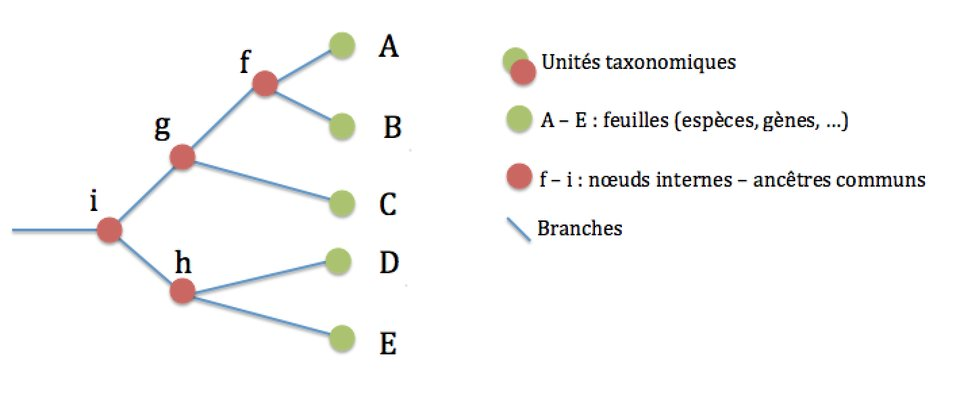
\includegraphics{Images/arbre_intro.jpg}(\url{http://zestedesavoir.com/media/galleries/2272/d1a1051e-782b-4b5d-81ac-c5641962b9c8.png.960x960_q85.jpg})
Dans la suite, nous nous intéresserons aux \emph{branchements évolutifs}.
Supposons qu'un branchement évolutif apparaît après une durée aléatoire d'une loi fixée \(\mu\) indépendamment du passé et du futur évolutif des espèces.\\
Quelle est cette loi \(\mu\)? Sa variance ? Sa moyenne ? \newline

\hspace*{0.5cm}

On observe des branchements successifs qui composent l'arbre
phylogénétique et à partir de ces données quantitatives observées, on
veut estimer la fonction de densité \(f\) qui donne la probabilité
qu'un nouveau branchement évolutif apparaisse après un certain temps.

Formellement on a le modèle de densité suivant: soient les variables aléatoires \(X_1,\dots,X_n\), \(n \in \mathbb{N^*}\) à valeur dans \(\mathbb{R}^d\) (ici \(d=1\)), indépendantes et identiquement distribuées de longueurs de branche observées. Elles ont pour fonction de densité \(f\) par rapport à la mesure de Lebesgue sur \(\mathbb{R}\) supposée inconnue. Notre objectif est d'estimer cette fonction densité \(f\) sur laquelle on fait le moins d'hypothèses possibles. On fera seulement les hypothèses d'existence, de continuité et de positivité de la fonction, en servant une observation \((X_1,...X_n)\), ce qui nous mène en statistique non-paramétrique, où le paramètre cherché est une densité de probabilité qui appartient à un espace fonctionnel infini, d'où la problématique de notre sujet.

\hypertarget{probluxe9matique}{%
\section{Problématique}\label{probluxe9matique}}

Comment estimer la loi de densité de la création d'une nouvelle espèce
avec une méthode d'estimation non-paramétrique ?

Pour commencer, en se basant sur quelques définitions nous présenterons les méthodes d'estimations non-paramétriques et en introduisant quelques types d'estimateurs.\newline
Par la suite, nous approfondirons les estimateurs de densité à noyau en menant une discussion sur leurs critères d'évaluation. Ainsi nous consacrerons un chapitre pour présenter des méthodes adaptatives.\newline
Enfin, pour répondre à la problématique, nous implémenterons un estimateur à noyau adaptatif, avec la méthode de validation croisée puis l'utiliserons sur des données d'arbres phylogénétiques.

\hypertarget{muxe9thodes-non-paramuxe9triques}{%
\chapter{Méthodes non-paramétriques}\label{muxe9thodes-non-paramuxe9triques}}

\hspace*{0.5cm} En statistique, on parle d'estimation quand on cherche à trouver certains paramètres inconnus caractérisant une distribution à partir d'un échantillon de données observées, en se basant sur différentes méthodes.
Dans notre cas, le paramètre d'intérêt est une fonction de densité appartenant à une classe fonctionnelle non fini-dimensionnelle. On se tourne vers l'estimation non-paramétrique lorsque l'on traite des paramètres non fini-dimensionnels.\\
\hspace*{0.5cm} Nous présenterons dans la suite une courte introduction
à l'estimation non-paramétrique et nous introduirons les deux classes
principales de l'estimation fonctionnelle : l'estimation par projection
et l'estimation à noyau.

\hypertarget{introduction}{%
\section{Introduction}\label{introduction}}

\hspace*{0.5cm}

L'estimation non-paramétrique vise à résoudre des problèmes d'estimation dans le cadre statistique où le modèle auquel on s'intéresse n'est pas décrit par un nombre fini de paramètres et dont chacun de ces paramètres ne permet pas de décrire la structure générale de la distribution des variables aléatoires.\newline Cela signifie qu'on utilise des modèles statistiques à dimension infinie.

\hspace*{0.5cm}

Dans le cadre de notre problématique on s'intéresse à l'estimation de densité.\newline
Un des principes de base de l'estimation de la densité selon une méthode d'estimation non-paramétrique est le suivant \newline

Soit un échantillon \(X=\{X_1, \dots,X_n\}\) de variables aléatoires réelles \(i.i.d.\) admettant une densité \(f = F'\), où \(F\) est une fonction de répartition. Supposons que \(f \in \mathcal F\) où \(\mathcal{F}\) est l'espace des fonctions positives, intégrables et d'intégrale égale à 1 sur \{\mathcal R\}. On cherche à estimer la fonction de densité inconnue \(f\) à partir de ces observations.\newline
On notera \(\hat f_n\) l'estimateur de \(f\).\newline
On se trouve donc avec le modèle suivant \(\{\mathbb P=\mathbb P_f,~f \in \mathcal F\}\)
où \(\mathbb P_f\) est la mesure probabilité de la densité \(f\).

L'estimation ici concerne donc la fonction elle même plutôt que les paramètres, ce qui explique le nom d'estimation non-paramétrique.\newline

\begin{rem}  
 On considère souvent les distances $L^p$ avec $p = 1,2$ ou $\infty$, si $f$ vérifie $\int_{\mathbb R} |f(x)|^p dx<+\infty$.
\end{rem}

\hspace*{0.5cm}

Nous traiterons dans la suite deux grandes familles de méthodes linéaires pour estimer une fonction densité : \newline
\hspace*{0.5cm} - L'estimation par projection, \newline
\hspace*{0.5cm} - L'estimation par noyau.

\hypertarget{estimateurs-par-projection}{%
\section{Estimateurs par projection :}\label{estimateurs-par-projection}}

\begin{dfn}
Soient $X= (X_1,...,X_n)$ un échantillon de densité $f$ et $T_j : \mathbb{R}^d \times \mathbb{R}^d \rightarrow \mathbb{R}$ des fonctions mesurables.  
Un estimateur $x \mapsto \hat{f}(x) = \hat{f}(x,X)$ est dit linéaire si il peut s'écrire sous la forme

$$
\hat{f}(x) = \sum^N_{j=1}T_j(x,X_j), \forall x \in \mathbb{R}^d.
$$

\end{dfn}

\begin{dfn}
(Estimateur par projection) \newline
Soit $f \in \mathcal F = (L^2 , \parallel\,.\parallel, <\,.,~.>)$ où $\mathcal{F} $ un espace de Hilbert muni d'une base orthonormée $(\Phi_j)_{j \in \mathbb{N^*}}$ de $L^2$.Si $\mathbb E _N$  un sous-espace vectoriel de dimension finie de $\mathcal F$ et $a_j = <f,\Phi_j> = \int_{\mathbb R}f(x)\Phi_j(x) dx$ avec $1 \leq |N| < \infty$.\newline
On appelle estimateur par projection de la fonction $f$ sur $\mathbb E_N$, la fonction $\Pi_N~f$ définit comme suit 

à modifier
$$
\Pi_{vect(1,..N)}~f = \sum_{j=1}^N a_j \Phi_j
$$
\end{dfn}

\begin{rem}
Cette méthode nous ramène au cas paramétrique.\newline
\end{rem}

\textbf{Exemple : l'estimation par histogramme}

\begin{exem}
  Une des premières approches possibles d'estimations non-paramétriques par projection de la fonction de densité est l'estimation par l'histogramme. C'est une méthode qui consiste à obtenir une segmentation de la répartition des observations par une projection sur une base constante par morceaux. L'histogramme est considéré comme une approximation discontinue de la fonction densité f.
  \label{eq:cours-est}

  
  (ajout formule graphique)
\end{exem}

Dans la suite on procédera à la méthode la plus fréquemment utilisée pour l'estimation d'une densité : L'estimation à noyau.\newline 

(Argument pour le choix de la méthode à voir)

\hypertarget{estimateurs-uxe0-noyau-de-densituxe9}{%
\section{Estimateurs à noyau de densité}\label{estimateurs-uxe0-noyau-de-densituxe9}}

Notre but est d'estimer la densité \(f\). Pour cela, on s'appuiera sur un échantillon \(i.i.d.\) \(X= (X_1,...,X_n)\) où chacune des variables \(X_i\) admet la densité \(f\) (par rapport à la mesure de Lebesgue).

Pour estimer une densité on peut utiliser une méthode à noyau.
Les méthodes à noyau sont des méthodes non-paramétriques qui permettent de proposer une estimation de la densité plus lisse que celle obtenue par un histogramme.

\begin{dfn} (Noyau)  

Un noyau (kernel en anglais) est une application $K:\mathbb{R}\rightarrow\mathbb{R}$ intégrable et centrée telle que :
$$\int_{\mathbb R} K(u) du = 1 ~~~~ \hbox{ et } ~~~~ \int_{\mathbb R} u K(u)=0$$
si le noyau est en plus positif alors il correspond à une fonction de densité.
\end{dfn}

\textbf{Comment construit-on un estimateur à noyau ?}

L'idée pour la construction de cet estimateur est d'utiliser l'approximation suivante , valable lorsque h est petit :\\
\[
f(x) = F'(x)\approx \frac{F(x+h)-F(x-h)}{2h}
\]
Pour estimer la densité \(f\) on peut passer par un estimateur \(\hat F_n\) de la fonction de répartition \(F\). \(\hat F_n\) est la fonction de répartition empirique ( \(\hat F_n(x)= \frac1n \sum\limits_{i=1}^n\frac{1}{2h} \mathds1_{X_i \in ]x-h, x+h[}\) ).
\[
\hat f_n(x)= \frac{\hat F_n(x+h)-\hat F_n(x-h)}{2h} = \frac 1n \sum\limits_{i=1}^n \frac1{2h} \mathds1_{X_i \in ]x-h;x+h]}
\]

Notons \(\hat f(x)\) l'estimateur à noyau de la densité \(f\), alors celui-ci s'écrit :
\[
\hat f_n(x) = \frac1{nh} \sum\limits_{i=1}^n K\left(\frac{X_i-x}h\right)
\]
où \(h\) est la fenêtre (ou paramètre de lissage), \(n\) le nombre d'observations, et \(K\) le noyau.
Cette formule n'est valable que si \(h\) est petit et strictement positif.

ici \(K(u)= \frac12 \mathds{1}_{u \in ]-1;1]}\), il s'agit du noyau de Rosenblatt, mais il existe d'autres noyaux.

Exemples de noyau :

\begin{itemize}
\item
  Noyau de Rosenblatt, ou rectangulaire : \(K(u)= \frac12 \mathds{1}_{u\in]-1;1]}\)
\item
  Noyau Gaussien : \(K(u) =\frac1{\sqrt{2\pi}}exp(-\frac{u^2}2)\)
\item
  Noyau d'Epanechnikov : \(K(u) =\frac34(1-u^2)\mathds{1}_{[-1,1]}(u)\)
\item
  Noyau triangulaire : \(K(u) = (1-\mid u \mid)\mathds{1}_{[-1,1]}(u)\)
\item
  Noyau Biweight : \(K(u) = \frac{15}{16}(1-u^2)^2\mathds{1}_{[-1,1]}(u)\)
\end{itemize}

Les propriétés du noyau (continuité, différentiabilité\ldots) se transmettent à l'estimateur \(\hat f_n\).

\begin{lem}  
Soient :\newline 
$h>0$ le paramètre de lissage et $K_h : u\in \mathbb{R} \rightarrow K(\frac{u}{h})/h$.On peut approximer la famille $(K_h)_{h>0}$ par l'identité du produit de convolution.
\end{lem}

\begin{demo}
A Faire
\end{demo}

\begin{corol}
$K_h * f : x \rightarrow \int_{\mathbb R} K_h(y-x) f(x) dx$ tend vers la fonction f quand h tend vers 0 pour la distance $L^2$.
\end{corol}

Après cette petite présentation de quelques estimateurs non-paramétriques de la densité, nous avons choisi de développer la partie sur l'estimation par noyau. c'est le type d'estimation que nous choisirons d'utiliser pour la suite de notre étude.

\hypertarget{estimateur-de-densituxe9-uxe0-noyau}{%
\chapter{Estimateur de densité à noyau}\label{estimateur-de-densituxe9-uxe0-noyau}}

\hypertarget{evaluer-un-estimateur}{%
\section{Evaluer un estimateur}\label{evaluer-un-estimateur}}

Avant de commencer cette partie on va d'abord introduire quelques notions et définitions\newline

\begin{dfn} {Noyau}  \newline
On note par le noyau la fonction intégrable K : $\mathbb{R}\rightarrow\mathbb{R}$ tel que:
$$\int_{\mathbb{R}}K(u)du =1.$$
\end{dfn}

\begin{lem}  
Soient :\newline 
$h>0$ le paramètre de lissage et $K_h : u\in \mathbb{R} \rightarrow K(\frac{u}{h})/h$.On peut approximer la famille $(K_h)_{h>0}$ par l'identité du produit de convolution.
\end{lem}

\begin{demo}
A Faire
\end{demo}

\begin{corol}
$K_h * f : x \rightarrow \int_{\mathbb R} K_h(y-x) f(x) dx$ tend vers la fonction f quand h tend vers 0 pour la distance $L^2$.
\end{corol}

Pour évaluer un estimateur \(\hat{f}\) on définit son risque associé.\newline 

\begin{dfn} 
La fonction de risque : 
$$ 
\mathcal R(\hat f ,f)=\mathbb E_f[\parallel\hat f -f\parallel^2]
$$
\end{dfn}

\begin{rem}
  La fonction de risque associé nous permet de comparer l'estimateur $\hat f$ et  f.\newline
On cherche à minimiser ce risque associé (i.e tend vers 0 pour un nombre d'observation assez grand).\newline
\end{rem}

\hypertarget{estimateur-de-densituxe9-uxe0-noyau-1}{%
\chapter{Estimateur de densité à noyau}\label{estimateur-de-densituxe9-uxe0-noyau-1}}

Dans un premier temps, nous cherchons à évaluer l'estimateur à noyau de densité. Pour cela nous allons utiliser la fonction de risque associée.

\hypertarget{risque-quadratique-des-estimateurs-uxe0-noyau-sur-les-classe-des-espaces-de-huxf6lder}{%
\section{Risque quadratique des estimateurs à noyau sur les classe des espaces de Hölder}\label{risque-quadratique-des-estimateurs-uxe0-noyau-sur-les-classe-des-espaces-de-huxf6lder}}

Nous nous intéressons au risque quadratique ponctuel de \(\hat{f}_n\), définit par :\\
étant donné \(x_0 \in \mathbb{R}\)
\[
R(\hat {f}_n, f) = \mathbb{E}[|\hat {f}_n(x_0) - f(x_0)|^2]
\]

\begin{rem}
  La fonction de risque associée nous permet de comparer l'estimateur $\hat f$ et  f.\newline
On cherche à minimiser ce risque associé (i.e tend vers 0 pour un nombre d'observations assez grand).\newline
\end{rem}

Rappelons la décomposition ``biais-variance'' du risque quadratique :
\[
\mathbb{E}[|\hat {f}_n(x_0) - f(x_0)|^2] = (\mathbb{E}[\hat {f}_n(x_0)] - f(x_0))^2 + \mathbb{V}[\hat {f}_n(x_0)]
\]

\hypertarget{majoration-du-biais-et-de-la-variance}{%
\subsection{Majoration du biais et de la variance}\label{majoration-du-biais-et-de-la-variance}}

Dans cette section, nous allons nous intéresser au compromis biais-variance afin de minimiser le risque quadratique.
Nous introduirons après quelques définitions deux propositions qui montrent que sous certaines hypothèses, on peut majorer le biais ainsi que la variance.\newline

\begin{dfn} Pour tout $\beta > 0$ et $L > 0$, on définit la classe de Hölder de régularité $\beta$ et de rayon $L$ par

$$
\begin{aligned}
  \Sigma(\beta,L)= ~\{&f:\mathbb{R} \longrightarrow \mathbb{R}\ \text{t.q.}\ f\ \text{est} \left\lfloor{\beta}\right\rfloor\ \text{fois dérivable et} \\
 & \forall\ (x,y) \in \mathbb{R}_2\ ~ \mid f^{\left\lfloor{\beta}\right\rfloor}(y)-f^{\left\lfloor{\beta}\right\rfloor}(x)\mid \leq L{\mid x-y\mid}^{\beta - \left\lfloor{\beta}\right\rfloor}\}
 \end{aligned}
$$

On notera $\Sigma_d(\beta,L)$ l'intersection de $\Sigma(\beta,L)$ et l'ensemble des densités.

\end{dfn}
\begin{rem} 
- Si $\beta = 1$ on obtient l'ensemble des fonctions L-lipschitziennes.\newline
- Si $\beta > 1$ alors $f'\in \Sigma(\beta-1,L)$.
\end{rem}
\begin{prop} (admise) Soit $\beta > 0$ et $L > 0$, il existe une constante $M(\beta, L)$ telle que

$$
\underset{f \in \Sigma_d(\beta,L)}{sup}{\parallel f \parallel}_{\infty}= \underset{x \in \mathbb{R}}{sup}\ \underset{f \in \Sigma_d(\beta,L)}{sup}f(x) \leq M(\beta,L)
$$
\end{prop}

\begin{dfn} Soit $\ell \in \mathbb{N^*}$. On dit que le noyau $K$ est d'ordre $\ell$ si $u^jK(u)$ est intégrable et 
$\int u^jK(u)du =  0,\   \ j = {1,...,\ell}$

\end{dfn}
\begin{prop}: Si $f \in \Sigma(\beta,L)$ avec $\beta > 0$ et $L > 0$ et si $K$ est un noyau d'ordre $\ell = \left\lfloor{\beta}\right\rfloor$ tel que $\int |{u}^{\beta}|\,.|{K(u)}|~du < \infty$ alors pour tout $x_0 \in \mathbb{R}$, et pour tout $h>0$ le biais peut être borné comme suit :

$$
|\mathbb{E}[\hat{f}_n(x_0)] - f(x_0)|\leqslant \frac{h^{\beta}L}{\ell!}\int|u|^{\beta}|K(u)|du
$$
\end{prop}

\begin{demo} On a
$$
\begin{aligned}
\mathbb E\lgroup \hat f_n(x_0) \rgroup&=\mathbb E\lgroup\frac{1}{n}\sum_{i=1}^n \frac{1}{h}K(\frac{X_i-x_0}{h})\rgroup \\
&=\mathbb E\lgroup \frac{1}{h}K(\frac{X_1-x_0}{h})\rgroup \\
&=\frac{1}{h}\int K(\frac{u-x_0}{h})f(u)du  \\
&=\int K(v)f(x_0+hv)dv,\  (en\ posant\ v=\frac{u-x_0}{h}).
\end{aligned}
$$
De plus
$$
f(x_0)=f(x_0)\times 1 = f(x_0) \int K(v)dv.
$$
Comme $f \in \Sigma(\beta, L)$, f admet $\left\lfloor{\beta} \right \rfloor$ dérivées et par un développement de Taylor-Lagrange on a, pour tout $x \in \mathbb R$,

$$
f(x)= \sum_{i=1}^{\ell-1}\frac{(x-x_0)^k}{k!}f^{(k)}(x_0)+\frac{(x-x_0)^\ell}{\ell!}f^{(\ell)}(x_0+\zeta (x-x_0))
$$  

avec $\zeta \in ]0,1[$. Autrement dit on a, avec $x= x_0+hv$,
$$
f(x_0+hv)-f(x_0)=\sum_{i=1}^{\ell-1}\frac{(hv)^k}{k!}f^{(k)}(x_0)+f^{(\ell)}(x_0+hv\zeta)\frac{(hv)}{\ell !}
$$  
pour un certain $\zeta \in ]0,1[$. Donc

$$
\begin{aligned}
\int K(v)\lgroup f(x_0+hv)-f(x_0)\rgroup dv &= \int K(v)\lgroup\sum_{i=1}^{\ell - 1}f^{(k)}(x_0)+f^{(\ell)}(x_0+hv\zeta)\frac{(hv)^{\ell}}{\ell !}\rgroup dv \\
&=\frac{h^{\ell}}{\ell !}\int K(v)v^{\ell}f^{(\ell)}(x_0+hv\zeta)dv
\end{aligned}
$$

Comme $K$ est d'ordre $\ell$, on a aussi $\int K(v)v^{\ell}f'^(\ell)(x_0)dv=0$. Donc on a
$$
\int K(v)\lgroup f(x_0+hv)-f(x_0)\rgroup dv = \frac{h^{\ell}}{\ell !}\int K(v)v^{(\ell)}\lgroup f^{(\ell)}(x_0 + hv\zeta)-f^{(\ell)}(x_0)\rgroup dv
$$
Or, $f \in \Sigma(\beta, L)$, on a donc $\mid f^{(\ell)}(x_0+hv\zeta)-f^{(\ell)}(x_0)\mid \leq L|hv|^{\beta-\ell}$. Et finalement
$$
\mid \int K(v)\lgroup f(x_0+hv\zeta)-f(x_0)\rgroup dv \mid \leq \frac{\mid h\mid^{\beta}}{\ell !}\int \mid K(v) \mid |v|^{\ell}l|hv|^{\beta-\ell}dv
$$

ce qui signifie que
$$
|\mathbb E \lgroup\hat f_n(x_0)-f(x_0)| \leq \frac{L|h|^{\beta}}{\ell !}\int |K(v)||v|^{\beta}dv
$$
\end{demo}
\begin{corol}   Le biais au carré tend vers zéro à la vitesse $h^{2\beta}$. En particulier, le biais tend vers zéro quand $h$ tend vers zéro. Plus la fonction $f$ est régulière, plus le biais tend vite vers zéro quand $h$ tend vers zéro (à condition bien sûr que l'ordre du noyau soit suffisamment grand). Nous en déduisons la convergence de l'espérance de l'estimateur à noyau $\hat {f}_n$ vers la fonction $f$. Et donc, l'estimateur à noyau est asymptotiquement sans biais, $\hat {f}_n$ est donc consistant.\newline
 \end{corol}
\begin{prop}: Si $f$ est bornée et si $K$ est de carré intégrable alors 

$$
\mathbb{V}(\hat {f}_n(x_0)) \leqslant \frac{\begin{Vmatrix}f\end{Vmatrix}_{\infty}\begin{Vmatrix}K\end{Vmatrix}^2_2}{nh}
$$

En particulier, si $f \in \Sigma(\beta,L)$ alors

$$
\mathbb{V}(\hat {f}_n(x_0)) \leqslant \frac{M(\beta, L)\begin{Vmatrix}K\end{Vmatrix}^2_2}{nh}
$$

\end{prop}
\begin{demo}:
$$
\begin{aligned}
\mathbb{V}(\hat {f}_n(x_0)) &= \mathbb{V}(\frac{1}{nh}\sum_{i=1}^nK(\frac{X_i-x_0}{h})) 
=\sum_{i=1}^n\mathbb{V}(\frac{1}{nh}K(\frac{X_i-x_0}{h})) \\
&=\sum_{i=1}^n\frac{1}{n^2h^2}\mathbb{V}(K(\frac{X_i-x_0}{h})) 
=\frac{1}{nh^2}\mathbb{V}(K(\frac{X_1-x_0}{h}) \\
&\leqslant \frac{1}{nh^2}\mathbb{E}(K^2(\frac{X_1-x_0}{h})) 
=\frac{1}{nh^2}\int K^2(\frac{u-x_0}{h})f(u)du \\
&\leqslant\frac{1}{nh}\int K^2(v)f(x_0 +vh)dv
\end{aligned}
$$ 

Et enfin,on utilise la proposition ? : il existe une constante positive $M(\beta,L)$ tel que $\begin{Vmatrix}f\end{Vmatrix}_{\infty} \leqslant M(\beta, L)$. Ceci implique que :
$$
 \mathbb{V}(\hat {f}_n(x_0))\leqslant\frac{1}{nh}M(\beta, L)\int K^2(v)dv 
$$ 
 \end{demo}

\begin{corol} Pour que la variance tende vers zéro, il faut que $nh$ tende vers l'infini. En particulier, à $n$ fixé, la variance est une fonction décroissante de $h$. Il y a donc une valeur optimale de $h$ qui doit réaliser l'équilibre entre le biais au carré et la variance. On peut à présent donner un contrôle du risque quadratique par le théorème suivant.
\end{corol}

\begin{thm} Soit $\beta>0$ et $L>0$ et $K$ un noyau de carré intégrable et d'ordre $\left\lfloor{\beta}\right\rfloor$ tel que $\int |u^{\beta}|\,.|K(u)|du<\infty$. Alors, en choisissant une fenêtre de la forme $h=cn^{-\frac{1}{2\beta+1}}$ avec une constante $c>0$, on obtient pour tout $x_0 \in \mathbb{R}$,

$$ 
R(\hat {f}_n(x_0)),\Sigma_d(\beta, L)):= \underset{f\in\Sigma_d(\beta,L)}{sup}\mathbb{E}[|\hat {f}_n(x_0)-f(x_0)|^2]\leqslant Cn^{-\frac{2\beta}{2\beta+1}}
$$ 
 où $C$ est une constante dépendant de $L,~\beta,~ c$ et $K$.
 \end{thm}
\begin{demo}
  On a :
$$
 R(\hat {f}_n(x_0),f(x_0))= \text{Biais}^2 + \text{Variance}
$$ 

Si nous nous référons aux deux propositions précédentes, nous pouvons écrire :
$$
 R(\hat {f}_n(x_0),f(x_0))\leqslant(\frac{h^{\beta}L}{l!}\int |u|^{\beta}|K(u)|du)^2 + \frac{M(\beta,L)\begin{Vmatrix}K\end{Vmatrix}_2^2}{nh}
$$

On cherche ensuite la fenêtre $h$ qui minimise cette quantité.Comme on cherche la vitesse de convergence en $h$, on utilisera la notation $c_1=(\frac{L}{l!}\int |u|^{\beta}|K(u)|du)^2$ et $c_2=M(\beta,L)\begin{Vmatrix}K\end{Vmatrix}_2^2$ qui ne dépendent pas de $h$. On doit alors minimiser en $h$ la quantité :
$$
  c_1h^{2\beta}+\frac{c_2}{nh}
$$

On a une somme d'une quantité croissante et une quantité décroissante en $h$. On cherche la fenêtre $h$ qui nous donne l'ordre minimal du risque. Quand $h$ est trop grand, le biais est trop grand, et quand $h$ est trop petit, c'est la variance qui est trop grande (voir exemple ci-dessous). On cherche donc la fenêtre $h$ qui réalise un équilibre entre le biais au carré et la variance:

$$ 
  h^{2\beta}\approx\frac{1}{nh}
$$
où le signe $\approx$ signifie ici "de l'ordre de". Cela donne :

$$
  h\approx n^{-\frac{1}{2\beta +1}}
$$

Autrement dit, pour une fenêtre $h$ de l'ordre de $n^{-\frac{1}{2\beta+1}}$, le biais au carré et la variance sont de même ordre.Plus exactement, on choisit la fenêtre $h_*=cn^{-\frac{1}{2\beta+1}}$, avec $c$ une constante strictement positive, on a :
$$
  \text{Biais au carré} \approx h_{*}^{2\beta}\approx \text{Variance} \approx \frac{1}{nh_{*}}
$$

De plus, on a alors :
$$
  h_* \approx n^{-\frac{2\beta}{2\beta + 1}}
$$

Autrement dit, il existe une certaine constante $C$ telle que, pour cette fenêtre $h_*$, on a :
$$
  R(\hat {f}_n(x_0),\sum_d(\beta,L))\leqslant Cn^{\frac{-2\beta}{2\beta + 1}}
$$

  Cette fenêtre est donc optimale à une constante près (si on change $c$, on change $C$ ça ne change pas le taux qui est $n^{\frac{-2\beta}{2\beta+1}}$).\newline
\end{demo}
\begin{cmtr}: L'estimateur dépend de $\beta$ à travers la fenêtre $h$. Or, sans   connaissance a priori sur les propriétés de la fonction $f$, on ne peut donc pas utiliser cet estimateur. On essaie alors de trouver un choix de fenêtre ne dépendant que des données et qui soit aussi performant (ou presque) que l'estimateur utilisant cette fenêtre optimale. A ce sujet, on introduira plus loin un choix de fenêtre ne dépendant que des données et qui est basé sur ce qu'on appelle la validation croisée (ou "cross validation" en Anglais).  \newline
\end{cmtr}

\textbackslash begin\{exem\} (Simulation numérique)
Nous estimons la fonction densité d'une somme de deux variables gaussiennes ci-contre avec la méthode à noyau avec différentes fenêtres.
\[
f(x)=\frac{1}{2}\frac{1}{\sqrt{2\pi}}(exp(-\frac{(x-2)^2}{2})+exp(-\frac{(x-6)^2}{2}))
\]
On va en fait utiliser \texttt{ggplot} pour représenter l'estimateur à noyau. La fonction qui permet de dessiner l'estimateur à noyau est \texttt{geom\_density}. Le paramètre représentant le fenêtre h rappelle \texttt{bw} (comme bandwidth en Anglais).
\textbackslash end\{exem\}

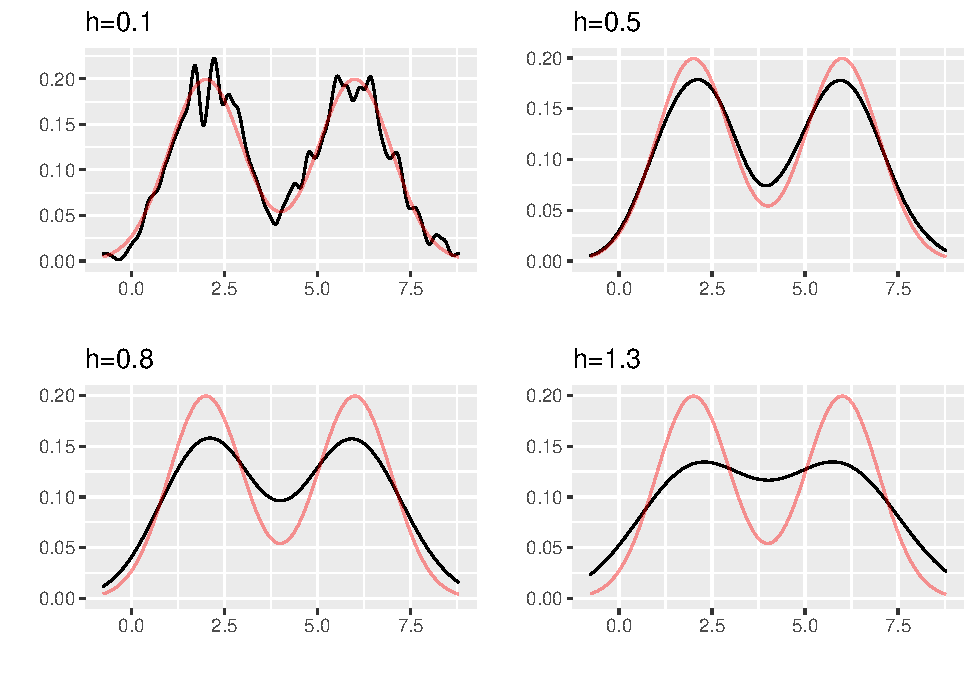
\includegraphics{Projet_M1_Chaoui_Manuel_Sadio_files/figure-latex/unnamed-chunk-2-1.pdf}

\hypertarget{muxe9thodes-adaptatives}{%
\section{Méthodes adaptatives}\label{muxe9thodes-adaptatives}}

\hspace*{0.5cm} On introduit précédemment la notion de l'estimation de la densité qui dépend d'un paramètre de lissage \(h\). Soit \((\hat{f_h})_{h\in \mathcal H}\) une famille des estimateurs de la fonction densité \(f\) que que l'on cherchons cherche à estimer.\newline
Une question s'impose : comment peut-on construire un estimateur à risque optimal à partir de cette famille en tenant en considération les observations ? \newline
Dans la théorie adaptative f est toujours supposée appartenir à une classe fonctionnelle. Cette classe n'est pas connu à priori mais supposé appartenir à une famille de classes fonctionnelles\{\(\mathcal{F_{\alpha}},\alpha \in\mathcal{A}\)\} où \(\mathcal{A}\) est un ensemble des paramètres de nuisance. ( ref : Sur l'estimation adaptative d'une densité multivariée sous l'hypothèse de la structure d'indépendance-Approche minimax adaptative).\newline

\hspace*{0.5cm} Dans cette partie, afin de répondre à la question posée auparavant, nous allons discuter du choix du noyau en premier lieu. Ensuite, nous introduirons deux méthodes pour le choix du paramètre de lissage \(h\).

\hypertarget{choix-du-noyau}{%
\subsection{Choix du noyau}\label{choix-du-noyau}}

\hspace*{0.5cm} Avant de présenter le critère de choix du noyau nous allons introduire quelques outils mathématiques qui simplifient l'écriture du critère.\\
Tout d'abord, nous avons besoin du risque quadratique \(\mathcal R\) aussi appelé l'erreur quadratique moyenne (\textbf{M}ean \textbf{S}quared \textbf{E}rror en anglais). Dans cette partie nous allons noter \(MSE\) le risque quadratique pour des questions pratiques.

\[
\begin{aligned}
MSE &= \mathcal R = \mathbb E \left[ \{  \hat f_n(x)-f(x) \} \right] \\
&=\mathbb V \left[ \hat f_n(x) \right] + Biais^2 \left[ \hat f_n(x) \right] \\
&= MSE(x ; n, h, K, f).
\end{aligned}
\]
comme nous l'avons montré précédemment. @ref\{\#holder\}

\begin{propri} (Biais ponctuel)
Pour tout $x$ fixé dans $\mathbb R$, le biais de l'estimateur $\hat f_n$ est donnée par l'équation suivante : 
$$Biais \left[ \hat f_n(x) \right] \approx \frac12h^2f''(x)\int_{\mathbb R} t^2K(t) dt.$$
\end{propri}

\begin{demo}
Démontrons la propriété du biais.
Rappelons que les variables aléatoires $\{ X_1,~\dots, ~X_n\}$ sont $i.i.d.$, alors
$$
\begin{aligned}
Biais  \left[ \hat f_n(x) \right] &= \mathbb E \left[ \hat f_n(x) \right] - f(x) \\
&= \mathbb E \left[ \frac1{nh} \sum\limits_{i=1}^n K\left(\frac{X_i-x}h\right) - f(x) \right] \\
&= \frac1{nh} \sum\limits_{i=1}^n \mathbb E \left[  K\left(\frac{X_i-x}h\right) \right] - f(x) ~\text{par linéarité de l'espérance} \\
&= \frac1{h} \mathbb E \left[  K\left(\frac{X_1-x}h\right) \right] - f(x) ~~~~~\text{car les } X_i \text{ sont }i.i.d.\\
&= \frac1{h} \int_{\mathbb R}  K\left(\frac{x_1-x}h\right) f(x_1)dx_1 - f(x).
\end{aligned}
$$

Procédons à un changement de variables.
$$t=\frac{x_1-x}h ~~~~\hbox{et}~~~~dt =\frac{dx_1}h.$$
On obtient alors, 
$$
Biais  \left[ \hat f_n(x) \right]
= \int_{\mathbb R}  K(t)  f(x+ht)dt - f(x).
$$

Après avoir transformé l'écriture du biais, nous pouvons donner une approximation de celui-ci en utilisant la formule de Taylor-Young à l'ordre 2.
$$f(x+ht)=f(x)+htf'(x)+\frac{h^2t^2}2 f''(x)+o(h^2t^2).$$
Ce qui nous donne en remplaçant dans la formule
$$
Biais \left[ \hat f_n(x) \right] \approx \frac12h^2f''(x)\int_{\mathbb R} t^2K(t) dt - f(x) + o(h^2t^2).
$$

et puisque le noyau est centré et son intégrale sur $\mathbb R$ est égale à $1$, on a bien que 
$$Biais \left[ \hat f_n(x) \right] \approx \frac12h^2f''(x)\int_{\mathbb R} t^2K(t) dt.$$

\end{demo}

\begin{propri} (Variance ponctuelle)
Pour tout $x$ fixé dans $\mathbb R$, la variance de l'estimateur $\hat f_n$ est donnée par l'équation suivante : 
$$\mathbb V \left[ \hat f_n(x) \right] \approx \frac1{nh} f(x) \int_{\mathbb R}K(t)^2 dt.$$
\end{propri}

\begin{demo}
Démontrons la propriété de la variance.
Rappelons que les variables aléatoires $\{ X_1,~\dots, ~X_n\}$ sont $i.i.d.$, alors
$$
\begin{aligned}
\mathbb V  \left[ \hat f_n(x) \right] &= \mathbb V \left[ \frac1{nh} \sum\limits_{i=1}^n K\left(\frac{X_i-x}h\right) \right] \\
&= \frac1{nh^2} \mathbb V \left[  K\left(\frac{X_1-x}h\right) \right] ~~~~~\text{car les } X_i \text{ sont }i.i.d.\\
&= \frac1{nh^2} \mathbb E \left[  K\left(\frac{X_1-x}h\right)^2 \right] - \frac1{nh^2} \mathbb E \left[  K\left(\frac{X_1-x}h\right) \right]^2\\
&= \frac1{nh^2} \int_{\mathbb R}  K^2\left(\frac{x_1-x}h\right) f(x_1)dx_1 - \frac1{nh^2} \left[\int_{\mathbb R}  K\left(\frac{x_1-x}h\right) f(x_1)dx_1\right]^2.
\end{aligned}
$$
On effectue encore une fois le même changement de variables.
$$t=\frac{x_1-x}h ~~~~\hbox{et}~~~~dt =\frac{dx_1}h.$$
Nous trouvons désormais,
$$
\begin{aligned}
\mathbb V  \left[ \hat f_n(x) \right] &= \frac1{nh} \int_{\mathbb R}  K^2\left(t\right) f(x+ht)dt - \frac1{n} \left[\int_{\mathbb R}  K\left(t\right) f(x+ht)dt\right]^2\\
&= \frac1{nh} \int_{\mathbb R}  K^2\left(t\right) f(x+ht)dt - \frac1{n} \left[Biais \left( \hat f_n(x) \right) +f(x)\right]^2\\
&= \frac1{nh} \int_{\mathbb R}  K^2\left(t\right) f(x+ht)dt - \frac1{n} \left[O \left( h^2 \right) +f(x)\right]^2.
\end{aligned}
$$
Donc si la condition $\int_{mathbb R}K(u)^2du<+\infty$ est vérifiée et que la taille de l'échantillon est importante, l'équation suivante est avérée : 
$$\mathbb V \left[ \hat f_n(x) \right] \approx \frac1{nh} f(x) \int_{\mathbb R}K(t)^2 dt.$$

\end{demo}

L'approximation de l'erreur quadratique (\textbf{A}verage of \textbf{M}ean \textbf{S}quared \textbf{E}rror en anglais) est donnée par l'équation suivante :\\
\[
AMSE(x)= \frac1{nh} f(x) \int_{\mathbb R}K(t)^2 dt + \left(\frac12h^2f''(x)\int_{\mathbb R} t^2K(t) dt \right)^2.
\]
Elle a été calculée à partir de la variance approchée et du biais approché.

L'erreur quadratique moyenne intégrée (\textbf{M}ean \textbf{I}ntregrated \textbf{S}quared \textbf{E}rror en anglais) est une mesure théorique communément utilisée pour évaluer la différence entre \(f\) et \(\hat f_n\). Pour l'évaluer on utilise l'erreur quadratique moyenne qu'on intègre sur le support \(\mathbb R\) de l'estimateur.
\[
\begin{aligned}
MISE(n,h,K,f) &= \int_{\mathbb R}MSE(x;n,h,K,f)dx\\
&= \int_{\mathbb R} \mathbb V\left[ \hat f_n(x) \right]  dx+ \int_{\mathbb R} Biais^2 \left[ \hat f_n(x) \right]dx
\end{aligned}
\]

De la même façon que nous l'avons fait avec l'erreur quadratique moyenne, nous allons calculer l'expression approchée de l'erreur quadratique moyenne (\textbf{A}verage of \textbf{M}ean \textbf{I}ntegrated \textbf{S}quared \textbf{E}rror en anglais).

\[
\begin{aligned}
AMISE(x)&= \frac1{nh} \int_{\mathbb R}f(x)dx \int_{\mathbb R}K(t)^2 dt + \frac14h^4 \int_{\mathbb R}f''(x)dx ~~\left(\int_{\mathbb R} t^2K(t) dt \right)^2\\
&= \frac1{nh} \int_{\mathbb R}K(t)^2 dt 
+ \frac14h^4 \int_{\mathbb R}f''(x)dx ~~\left(\int_{\mathbb R} t^2K(t) dt \right)^2\\
&= \frac1{nh} \int_{\mathbb R}K(t)^2 dt 
+ \frac14h^4 ~ \mathbb V (K)^2 \int_{\mathbb R}f''(x)dx 
\end{aligned}
\]

\hspace*{0.5cm} à présent que nous avons défini les outils nécessaires au choix du noyau, nous allons pouvoir présenter un critère de choix pour les noyaux continus symétriques. Afin de mesurer l'efficacité des noyaux, nous utilisons une mesure qui calcule le rapport du critère \(AMISE\) de deux noyaux.
\[
eff(K_1,K_2) = \frac{AMISE(K_1)}{AMISE(K_2)}.
\]
Supposons que \(K_1\) est le noyau d'Epanechnikov, il est souvent utilisé comme référence par rapport aux autres noyaux continus. Après quelques calculs, on obtient que l'efficacité d'un noyau K par rapport à celui d'Epanechnikov est donnée par
\[
eff(K) = \frac{3}{5\times \int_{\mathbb R}K(t)^2 dt\sqrt{5 \times\int_{\mathbb R}t^2K(t) dt} } \leq1.
\]
Voici un tableau récapitulatif de l'efficacité de plusieurs noyaux continus symétriques.

\textbackslash begin\{table\}

\textbackslash caption\{(\#tab:ker\_tab)Efficacité des noyaux continus symétriques\}
\centering

\begin{tabular}[t]{l|r}
\hline
Noyau & Efficacité\\
\hline
Epanechnikov & 1.000\\
\hline
Bigweight & 0.994\\
\hline
Triangular & 0.986\\
\hline
Gaussien & 0.951\\
\hline
Rectangulaire & 0.930\\
\hline
\end{tabular}

\textbackslash end\{table\}

\begin{rem}
Les valeurs d'efficacité des noyaux sont très proches les unes des autres dans le cas étudié, surtout pour les trois premiers noyaux du tableau. c'est pour cela que le choix du noyau n'a au final que peu d'importance dans l'estimation de la densité. 
\end{rem}

\hypertarget{comment-choisir-les-paramuxe8tres-de-la-muxe9thode}{%
\subsubsection{Comment choisir les paramètres de la méthode ?}\label{comment-choisir-les-paramuxe8tres-de-la-muxe9thode}}

Dans la méthode d'estimation à noyau le choix du noyau n'est pas le plus important, le vrai enjeu de cette méthode est le choix de la fenêtre \(h\) (\emph{bandwidth}).
En effet, la fenêtre détermine l'influence des données dans l'estimation. Si \(h\) est petit, l'effet local est important donc on aura beaucoup de bruit. Si \(h\) est grand, on aura une estimation plus douce, plus lisse.

Nous pouvons constater l'influence du paramètre \(h\) sur l'exemple suivant :

Nous avons simulé 500 variables suivant une loi de Weibull de paramètres (\(\alpha = 1.7\), \(\lambda=2\)) représentées dans l'histogramme. La courbe en rouge est la fonction de densité de la loi de Weibull et la bleue est l'estimation avec la méthode des noyaux sur les variables simulées.

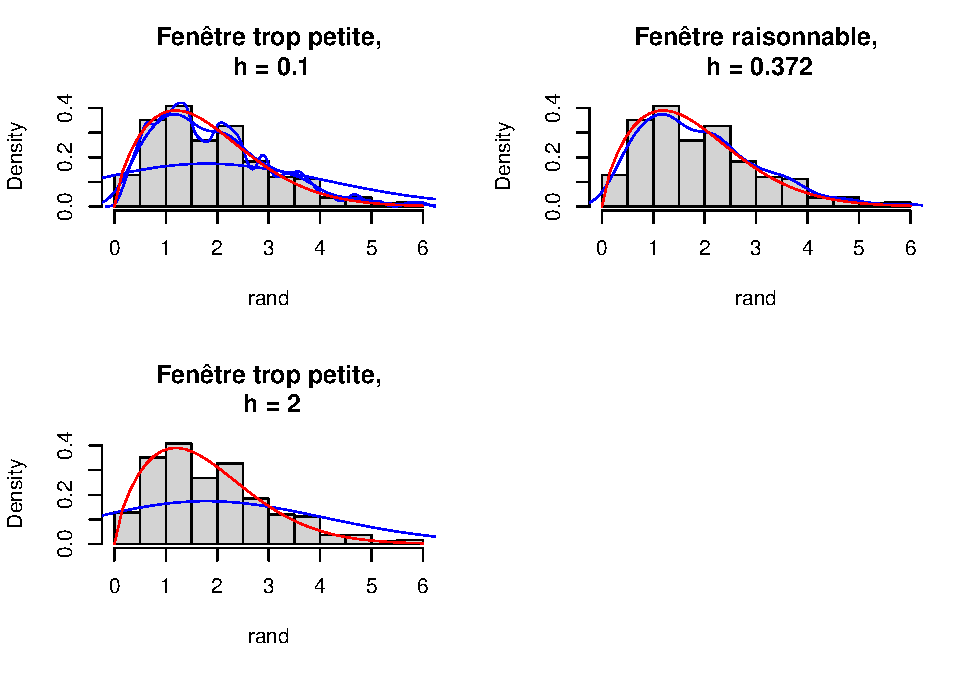
\includegraphics{Projet_M1_Chaoui_Manuel_Sadio_files/figure-latex/unnamed-chunk-3-1.pdf}
La fenêtre \(h\) du second graphique est calculée automatiquement par la fonction \texttt{density}de R.

\hypertarget{choix-de-la-fenuxeatre}{%
\subsection{Choix de la fenêtre}\label{choix-de-la-fenuxeatre}}

L'estimation de densité nécessite le choix de la fenêtre qu'on note h.\newline En statistique non-paramétrique, ils existent plusieurs méthodes et critères de qualité pour le choix de la fenêtre.\newline

On présente dans la suite deux méthodes:\newline
\hspace*{0.5cm} Méthode de validation croisée.\newline
\hspace*{0.5cm} Méthode de Goldenshluger-Lepski.\newline

\hypertarget{choix-de-la-fenuxeatre-h-par-validation-croisuxe9e}{%
\subsubsection{\texorpdfstring{Choix de la fenêtre \(h\) par validation croisée}{Choix de la fenêtre h par validation croisée}}\label{choix-de-la-fenuxeatre-h-par-validation-croisuxe9e}}

Le choix de la fenêtre dans la section précédente est critiquable: comme on l'a mentionné, il dépend de la régularité la fonction \(f\) qui est inconnue dans notre cas. On peut donc essayer d'estimer cette fenêtre idéale par un estimateur \(\hat{h}\). De façon à souligner la dépendance à la fonction, on va noter \(\hat{f}_{n,h}\) l'estimateur associé à un choix de fenêtre \(h\). L'estimateur final sera \(\hat{f}_{n,\hat{h}}\), une fois le choix de \(\hat{h}\) fait.\newline 

On cherche à minimiser en \(h\) le risque quadratique pour la distance \(L_2\) :
\[
\begin{aligned}
R(\hat {f}_{n,h})&=\mathbb{E}[\begin{Vmatrix}\hat {f}_{n,h}-f\end{Vmatrix}_2^2]\\        
&= \mathbb{E}[\begin{Vmatrix}\hat {f}_{n,h}\end{Vmatrix}_2^2] -2~\mathbb{E}[\int \hat {f}_{n,h}(x)f(x)dx] +\begin{Vmatrix}f\end{Vmatrix}_2^2
\end{aligned}
\]

Or la fonction \(f\) étant inconnue, ce risque n'est pas calculable à partir des données. On cherche donc à estimer ce risque en utilisant uniquement les données. Remarquons que minimiser en \(h\) la quantité \(R(\hat {f}_{n,h}, f)\) est équivalent à minimiser en \(h\) la quantité \(R(\hat {f}_{n,h}, f)-\begin{Vmatrix}f\end{Vmatrix}_2^2\). On va en fait remplacer la minimisation de la quantité inconnue \(R(\hat {f}_{n,h}, f)-\begin{Vmatrix}f\end{Vmatrix}_2^2\) par la minimisation d'un estimateur \(\hat {R}(h)\) de cette quantité. Plus précisément on va chercher un estimateur sans biais de cette expression:

\[
\mathbb{E}[\begin{Vmatrix}\hat {f}_{n,h}\end{Vmatrix}_2^2] -2~\mathbb{E}[\int \hat {f}_{n,h}(x)f(x)dx]
\]

Le premier terme admet \(\begin{Vmatrix}\hat {f}_{n,h}\end{Vmatrix}_2^2\) comme estimateur trivial (d'après la propriété des estimateurs sans biais : \(\mathbb{E}[\hat {\beta}]=\beta\)).\newline
Il reste à trouver un estimateur sans biais du second terme.

\begin{lem} Soit $\hat {G}$ définit en tout points sauf en $X_i$ (c'est le principe du Leave-one-out):

$$
\hat{G} = \frac{1}{n}\sum_{i=1}^n\hat {f}_{n,h}^{(-i)}(X_i)
$$
avec :

$$
  \hat {f}_{n,h}^{(-i)}(x)= \frac{1}{n-1}\frac{1}{h}\sum_{j=1,j\ne i}^nK(\frac{x-X_j}{h})
$$
Cette estimateur $\hat G$, par construction est l'estimateur sans biais de $\int \hat{f}_{n,h}(x)f(x)dx$.
\end{lem}
\begin{demo}
Montrons que $\mathbb{E}(\hat{G})=\mathbb{E}[\int \hat{f}_{n,h}(x)f(x)dx]$.\newline
Comme les $X_i$ sont i.i.d., d'une part nous avons :
$$
\begin{aligned}
\mathbb{E}[\int \hat {f}_{n,h}(x)f(x)dx]&= \mathbb{E}[\int \frac {1}{nh}\sum_{i=1}^nK(\frac {x-X_i}{h})f(x)dx]\\
&=\frac{1}{h}\mathbb{E}[\int K(\frac {x-x_1}{h})f(x)dx] \\
&=\frac{1}{h}\int f(x)\int K(\frac {x-X_1}{h})f(x_1)dx_1dx
\end{aligned}
$$
D'autre part, nous avons : 
$$ 
\begin{aligned}
\mathbb{E}[\hat{G}]&=\mathbb{E}[\frac{1}{n}\sum_{i=1}^n\hat{f}_{n,h}^{(-i)}(X_i)]
=\mathbb{E}[\hat{f}_{n,h}^{(-1)}(X_1)]\\
&=\mathbb{E}[\frac{1}{(n-1)h}\sum_{j\ne 1}K(\frac{X_j-X_1}{h})]\\
&=\mathbb{E}[\frac{1}{h}K(\frac{X-X_1}{h})]\\
&=\frac{1}{h}\int f(x)\int K(\frac{x-x_1}{h})f(x_1)dx_1dx\\
&=\mathbb{E}[\int \hat{f}_{n,h}(x)f(x)dx] 
\end{aligned}
$$

Donc, $\hat{G}$ est un estimateur sans biais de $\int\hat{f}_{n,h}(x)f(x)dx$.
\end{demo}

Finalement, l'estimateur sans biais de \(R(\hat{f}_{n,h}, f)-\begin{Vmatrix}{f}\end{Vmatrix}_2^2\) est donné par:

\[
\hat{R}(h)=\begin{Vmatrix}\hat{f}_{n,h}\end{Vmatrix}_2^2-\frac{2}{n(n-1)}\sum_{i=1}\sum_{j=1,j\ne i}\frac{1}{h}K(\frac{X_i-X_j}{h})
\]

On définit alors

\[
\hat{h} = arg\ \underset{h\in H}{min}\hat{R}(h)
\]

Si ce minimum est atteint. On cherche une fenêtre parmi une grille finie de valeurs, grille qu'on a notée \(H\) dans la formule ci-dessus.\\
L'estimateur \(\hat{f}_{n,\hat{h}}\) a de bonnes propriétés pratiques et de consistance.

La validation croisée est une méthode très générale mais nous l'utilisons ici pour le choix la fenêtre \(h\) optimale.

\hypertarget{muxe9thode-de-goldenshluger-lepski}{%
\subsubsection{Méthode de Goldenshluger-Lepski}\label{muxe9thode-de-goldenshluger-lepski}}

La méthode de Goldenshluger-Lepski donne principalement des critères de sélection dans une famille d'estimateurs linéaires à noyau, afin d'obtenir un estimateur vérifiant une inégalité d'oracle.\\
Avant de présenter ces critères de sélection, commençons d'abord par une introduction aux inégalités d'oracle dans l'estimation adaptative.

\hypertarget{inuxe9galituxe9s-doracle}{%
\paragraph{Inégalités d'oracle}\label{inuxe9galituxe9s-doracle}}

References pour cette partie.\label{eq:oracle} et \label{eq:est-ad} \newline
Supposons que la fonction estimée appartient à une classe fonctionnelle \(\mathcal{F}\) et qu'on a un nombre d'observations n fixé.\\
On a pour objectif de choisir, dans une famille d'estimateurs \(\mathbb{F} =\)\{\(\hat{f}_h ; h\in \mathcal{H}\)\} indexée par le paramètre \(h \in \mathcal{H}\), un estimateur \(\hat{f}_{h^*}\) qui soit le meilleur possible.\\
Cela revient à résoudre le problème de minimisation
\[
h^*=arg~inf_{h \in \mathcal{H}} R(\hat{f}_h,f)
\]
L'estimateur \(\hat{f}_{h^*}\) n'est pas calculable en pratique puisqu'il dépend de la fonction inconnue \(f\). C'est aussi pourquoi il est souvent appelé oracle. Le but est donc de se servir de son risque pour trouver un estimateur qui fonctionne presque comme cet oracle. Pour cela nous utilisons l'échantillon des observations pour sélectionner un paramètre \(\hat{h} \in \mathcal{H}\) tel que \(\hat{f}_{\hat{h}}\) vérifie une égalité d'oracle
\[
\mathcal{R}(\hat{f}_{\hat{h}},f) \leq C~inf_{h\in \mathcal{H}}~\mathcal{R}(\hat{f}_{h},f)+\delta,~~~~\forall~~f \in \mathcal{F}.
\]
où \(C \geq 1\) est une constante indépendante de n et de f, \(inf_{h\in \mathcal{H}}R(\hat{f}_h,f)\) est le risque d'oracle et \(\delta\) un terme résiduel indépendant de f, souvent négligeable devant le risque d'oracle.\\

\begin{rem}
Lorsque C vaut 1, l'inégalité est dite exacte et $\hat{f}_{\hat{h}}$ imite l'oracle sur $\mathcal{H}$. \newline
Lorsque C > 1, l'estimateur imite seulement la vitesse de convergence de l'oracle.\newline
Parfois quand il est difficile de comparer le risque de l'estimateur sélectionné avec celui de l'oracle. on cherche à obtenir une inégalité d'oracle
$$
\mathcal{R}(\hat{f}_{\hat{h}},f) \leq inf_{h \in \mathcal{H}}\mathcal{R}(h,f)+\delta,~~~~\forall~~f \in \mathcal{F}.
$$
 Avec $\mathcal{R}(h,f)$ une approximation du risque $\mathcal{R}(\hat{f}_{h},f)$ 
\end{rem}

La question qui se pose dans la suite est \newline
Soit \(\mathcal{F}\) une collection d'estimateurs construits à partir des données et \(\hat{f}_h \rightarrow \mathcal{R}(\hat{f}_h,f)\) un risque pour l'estimation de f, comment construire un estimateur \(\hat{f}_{\hat h}\) tel que \(\mathcal{R}(\hat{f}_{\hat h},f) \approx~~inf_{h \in \mathcal{H}} \mathcal{R}(\hat{f}_h,f)\) où \(\mathbb{E}[\mathcal{R}(\hat{f}_{\hat{h}},f)] \approx inf_{h \in \mathcal {H}} \mathbb{E}[\mathcal{R}(\hat{f}_h,f)]\)?
C'est là que s'applique la méthode de Goldenshluger et Lepski. Il s'agit une des méthodes usuelles qui imite la décomposition biais-variance du risque de l'estimateur. \newline
Cette méthode se base sur l'observation. Elle consiste à choisir un estimateur dans une famille d'estimateurs linéaires \(\mathbb{F} =\)\{\(\hat{f}_h,h \in \mathcal{H}\)\}. Pour cela on doit imposer d'abord quelques suppositions. \newline
\emph{Suppositions} \newline
-1) Le noyau K est lipschitzienne\newline

\[
|K(x)~-~K(y)| \leq c|x-y|,~~~~\forall(x,y)\in \mathbb{R}.
\]
OÙ \textbar.\textbar{} est la distance euclidienne.\newline
-2)Il existe un réel \(k_{\infty}<\infty\) tel que \(||K||_{\infty} \leq k_{\infty}\)

Passons ensuite au critère de sélection.\newline
\emph{Critère de sélection} \newline
Ce critère comme abordé au dessus se base sur la comparaisons des estimateurs deux à deux en faisant intervenir des estimateurs auxiliaires \{\(\hat f_{h,\mu},h~~ et~~ \mu \in \mathcal{H}\)\} définies comme suit
\[
\hat f_{h,\mu}(x)=\frac{1}{n}\sum^n_{i=1}[K_h * K_{\mu}](x-X_i),
\]
où * est le produit de convolution sur \(\mathbb{R}\).\newline
On définit aussi\newline
\[
\forall h \in \mathcal{H}~~\hat{\mathcal R}_h = sup_{\mu \in \mathcal{H}}[||\hat f_{h,\mu}-\hat f_\mu ||_s - m_s(h,\mu)]_+ + m^*_s(h),
\]
où la fonction \(m_s\) est appelé le majorant et \(m^*_s(h) = sup_{\mu \in \mathcal{H}}m_s(h,\mu) ~~ \forall h \in \mathcal{H}\)\newline

\begin{prop}
Soient $\xi_{h,\mu}$ et $\xi_\mu$ les erreurs stochastiques relatives aux estimateurs $\hat f_{h,\mu}$ et $\hat f_\mu$.\newline
La fonction $m_s$ est une majorante uniforme de la perte aléatoire$||\xi_{h,\mu}-\xi_\mu||_s$
\end{prop}
\begin{demo}
BANDWIDTH SELECTION IN KERNEL DENSITY ESTIMATION:
ORACLE INEQUALITIES AND ADAPTIVE MINIMAX
OPTIMALITY By ALEXANDER GOLDENSHLUGER1 AND OLEG LEPSKI
\end{demo}

\begin{rem}
La fonction majorante $m_s$ ne dépend pas de la fonction densité f.
\end{rem}

De tout ce qui précède \(\hat h\) est définie par\newline

\[
\hat h = arg~inf_{h \in \mathcal{H}} \mathcal{\hat R}_h.
\]

Et le critère de comparaison

\[
\hat{\Delta}(h)= sup_{\mu \in \mathcal{H}}[||\hat f_{h,\mu}-\hat f_\mu||_s - m_s(h,\mu)]_+,~~~~\forall h,\mu \in \mathcal H,~~\forall \hat f \in \mathbb F.
\]

\begin{rem}
Soient h et$\mu \in \mathcal H$, $m_s$ la fonction majorante définie auparavant et $\hat f \in \mathbb F$
$m_s$ est de l'ordre de l'écart type de $|\hat f_{h,\mu}(x)-\hat f_\mu(x)|$ pour tout x dans $\mathbb R$.
\end{rem}

Donc si l'inégalité suivante est vérifiée

\[
sup_{h \in \mathcal{H}}(\mathbb{E}_f~sup_{\mu \in \mathcal H}[||\xi_{h,\mu}-\xi_\mu || - m_s(h,\mu)]_+^2)^{\frac{1}{2}} \leq \delta,~~\forall f \in \mathbb{F}, ~~\forall h,\mu \in \mathcal H.
\]
Et si il existe \(\hat h \in \mathcal{H}\) mesurable par rapport à l'observation et vérifiant

\[
\hat{\Delta}(\hat h)+sup_{\mu \in \mathcal H}m_s(\hat h, \mu) \leq inf_{h \in \mathcal H}(\hat \Delta(h) +sup_{\mu \in \mathcal H}m_s(h,\mu)).
\]
Alors l'estimation sectionnée est \(\hat f_{\hat h}\).

\hypertarget{applications}{%
\chapter{Applications}\label{applications}}

Rappelons que nous cherchons à estimer la fonction de densité \(f\) de la durée avant la création d'une nouvelle espèce. Dans ce cadre nous allons faire nos estimations à noyau de la densité sur R en appliquant la théorie que nous avons vue jusque là.

\hypertarget{fonction-dens}{%
\section{Fonction dens}\label{fonction-dens}}

Dans cette partie nous présenterons la fonction \texttt{dens} que nous avons créée en voulant reproduire ce que fait la fonction \texttt{density} de R.
Voici son code :

Insérer le script de fonc\_dens.R

\hypertarget{applications-aux-donnuxe9es-du-vivant}{%
\section{Applications aux données du vivant}\label{applications-aux-donnuxe9es-du-vivant}}

Maintenant que nous avons notre fonction \texttt{dens} nous allons pouvoir la comparer à la fonction \texttt{density} de R. Pour les comparer nous allons en profiter pour en même temps les appliquer aux données qu'on veut étudier.

Pour commencer nous allons tester les fonctions avec un premier exemple fictif.

\begin{Shaded}
\begin{Highlighting}[]
\CommentTok{# Estimation de la densité par la méthode des noyaux (Test)}

\CommentTok{## Chi 2 à 6 ddl}

\NormalTok{seq <-}\StringTok{ }\KeywordTok{seq}\NormalTok{(}\DecValTok{0}\NormalTok{,}\DecValTok{30}\NormalTok{, }\DataTypeTok{length.out =} \DecValTok{60}\NormalTok{)}
\NormalTok{ychi2 <-}\StringTok{ }\KeywordTok{dchisq}\NormalTok{(seq,}\DecValTok{6}\NormalTok{)}
\CommentTok{#plot(seq, ychi2, type = "l", col = "red")}

\NormalTok{rand <-}\KeywordTok{rchisq}\NormalTok{(}\DecValTok{100}\NormalTok{,}\DecValTok{6}\NormalTok{)}
\KeywordTok{hist}\NormalTok{(rand, }\DataTypeTok{breaks =} \DecValTok{60}\NormalTok{, }\DataTypeTok{freq =}\NormalTok{ F, }\DataTypeTok{xlim=}\KeywordTok{c}\NormalTok{(}\DecValTok{0}\NormalTok{, }\KeywordTok{max}\NormalTok{(rand)}\OperatorTok{+}\DecValTok{3}\NormalTok{))}
\KeywordTok{lines}\NormalTok{(}\KeywordTok{density}\NormalTok{(rand, }\DataTypeTok{kernel =}  \StringTok{"epanechnikov"}\NormalTok{, }\DataTypeTok{bw =} \DecValTok{1}\NormalTok{), }\DataTypeTok{col =}\StringTok{"black"}\NormalTok{)}
\KeywordTok{lines}\NormalTok{(}\KeywordTok{density}\NormalTok{(rand),}\DataTypeTok{col=}\StringTok{"blue"}\NormalTok{)}
\KeywordTok{lines}\NormalTok{(}\KeywordTok{density}\NormalTok{(rand, }\DataTypeTok{kernel =}  \StringTok{"rectangular"}\NormalTok{), }\DataTypeTok{col =}\StringTok{"purple"}\NormalTok{)}
\KeywordTok{lines}\NormalTok{(}\KeywordTok{density}\NormalTok{(rand, }\DataTypeTok{kernel =}  \StringTok{"triangular"}\NormalTok{), }\DataTypeTok{col =}\StringTok{"green"}\NormalTok{)}
\KeywordTok{lines}\NormalTok{(seq, ychi2, }\DataTypeTok{col =} \StringTok{"red"}\NormalTok{)}
\KeywordTok{legend}\NormalTok{(}\StringTok{"topright"}\NormalTok{,}\KeywordTok{c}\NormalTok{(}\StringTok{"gaussien"}\NormalTok{, }\StringTok{"epanechnikov"}\NormalTok{, }\StringTok{"rectangulaire"}\NormalTok{, }\StringTok{"triangulaire"}\NormalTok{, }\StringTok{"chi2"}\NormalTok{),}
       \DataTypeTok{lty=}\DecValTok{1}\NormalTok{, }\DataTypeTok{col =} \KeywordTok{c}\NormalTok{(}\StringTok{"blue"}\NormalTok{, }\StringTok{"black"}\NormalTok{,}\StringTok{"purple"}\NormalTok{,}\StringTok{"green"}\NormalTok{,}\StringTok{"red"}\NormalTok{))}
\KeywordTok{rug}\NormalTok{(rand,}\DataTypeTok{col=}\StringTok{"darkred"}\NormalTok{) }\CommentTok{# Visualisation 1d}
\end{Highlighting}
\end{Shaded}

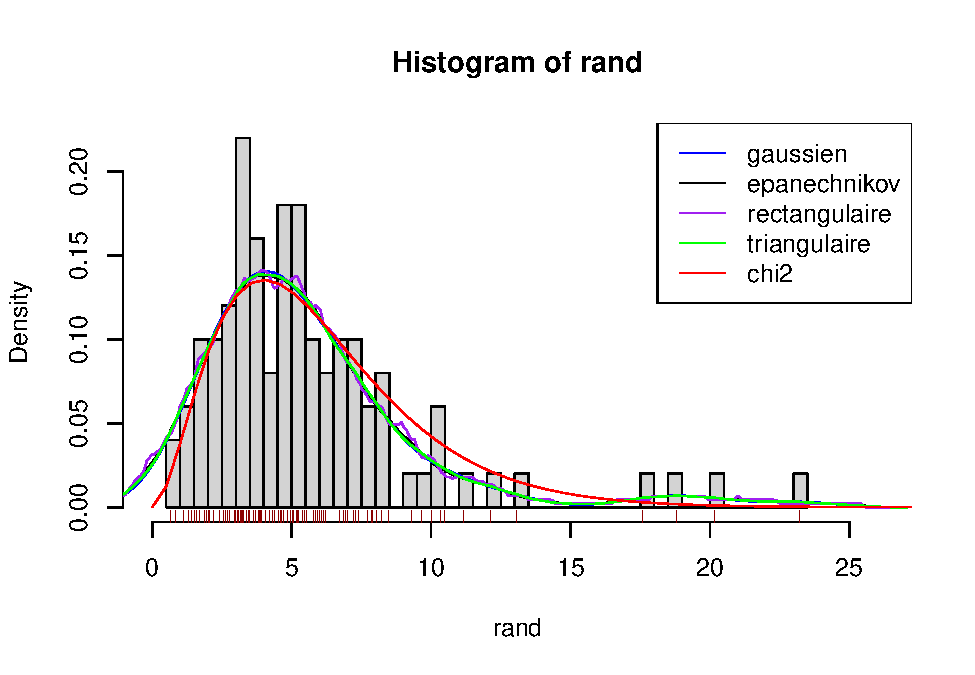
\includegraphics{Projet_M1_Chaoui_Manuel_Sadio_files/figure-latex/chi2-1.pdf}
Comme nous l'avons vu théoriquement, on voit relativement bien ici que la différence au niveau du choix du noyau n'est pas très impactante sur la qualité de l'estimation.

Nous allons maintenant tester les fonctions d'estimation de la densité sur deux exemples.
Commençons par les familles d'oiseaux (\texttt{bird.families}.

\begin{Shaded}
\begin{Highlighting}[]
\CommentTok{# Voici des librairies contenant des arbres phylogénétiques.}
\KeywordTok{library}\NormalTok{(ape)}
\KeywordTok{library}\NormalTok{(geiger)}

\CommentTok{## test avec bird families}

\CommentTok{### arbre}
\KeywordTok{data}\NormalTok{(}\StringTok{"bird.families"}\NormalTok{)}
\NormalTok{op <-}\StringTok{ }\KeywordTok{par}\NormalTok{()}
\KeywordTok{par}\NormalTok{(}\DataTypeTok{cex =} \FloatTok{0.3}\NormalTok{)}
\KeywordTok{plot}\NormalTok{(bird.families)}
\end{Highlighting}
\end{Shaded}

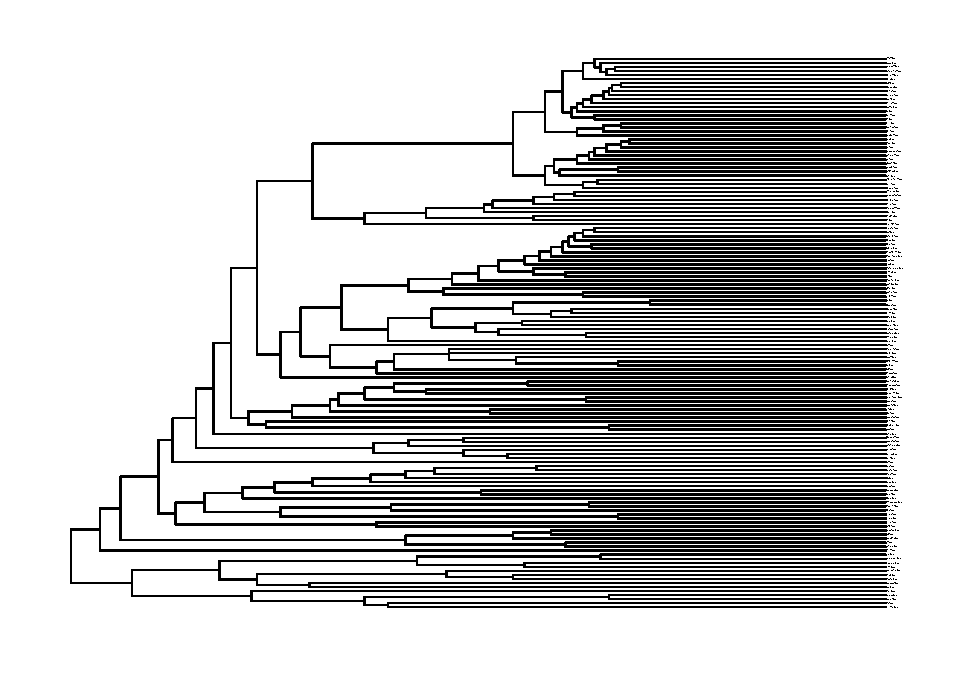
\includegraphics{Projet_M1_Chaoui_Manuel_Sadio_files/figure-latex/birds-1.pdf}

\begin{Shaded}
\begin{Highlighting}[]
\KeywordTok{par}\NormalTok{(}\DataTypeTok{cex =}\NormalTok{ op}\OperatorTok{$}\NormalTok{cex)}

\CommentTok{#### noyau gaussien}

\NormalTok{d<-bird.families}\OperatorTok{$}\NormalTok{edge.length}
\NormalTok{vec <-}\StringTok{ }\KeywordTok{pretty}\NormalTok{(}\DecValTok{0}\OperatorTok{:}\NormalTok{(}\KeywordTok{max}\NormalTok{(d)}\OperatorTok{+}\DecValTok{3}\NormalTok{),((}\KeywordTok{max}\NormalTok{(d)}\OperatorTok{+}\DecValTok{3}\NormalTok{)}\OperatorTok{*}\DecValTok{2}\NormalTok{))}
\KeywordTok{hist}\NormalTok{(d, }\DataTypeTok{breaks =}\NormalTok{ vec, }\DataTypeTok{freq =}\NormalTok{ F, }\DataTypeTok{xlab =} \StringTok{"Durée"}\NormalTok{)}
\KeywordTok{lines}\NormalTok{(}\KeywordTok{density}\NormalTok{(d), }\DataTypeTok{col =} \StringTok{"red"}\NormalTok{) }\CommentTok{# bw = 1.82}
\end{Highlighting}
\end{Shaded}

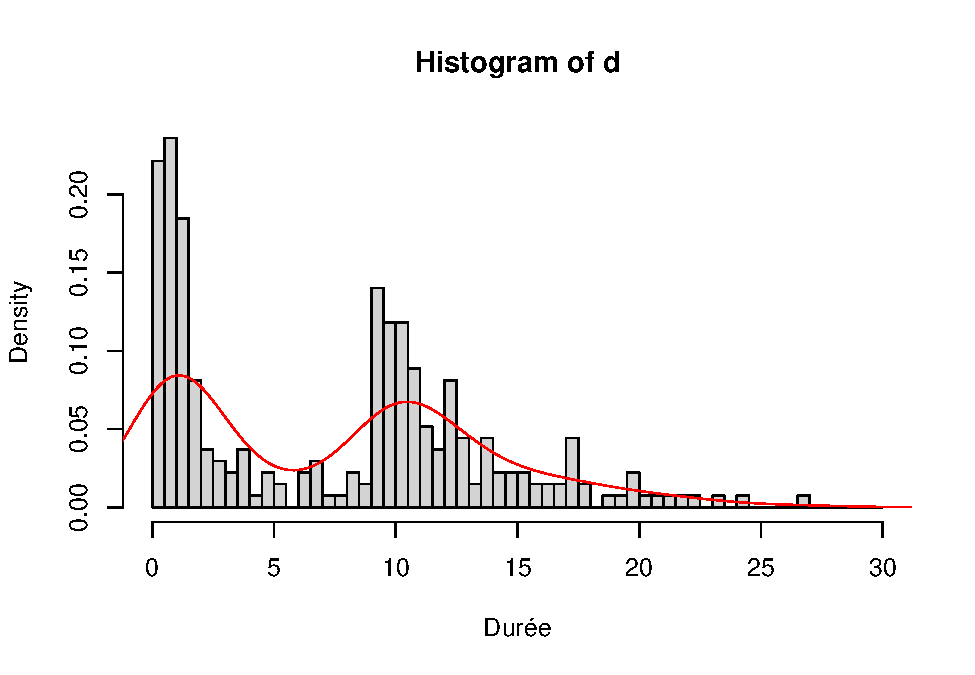
\includegraphics{Projet_M1_Chaoui_Manuel_Sadio_files/figure-latex/birds-2.pdf}

\begin{Shaded}
\begin{Highlighting}[]
\KeywordTok{plot}\NormalTok{(}\KeywordTok{density}\NormalTok{(d, }\DataTypeTok{kernel=} \StringTok{"gaussian"}\NormalTok{, }\DataTypeTok{window =} \StringTok{"gaussian"}\NormalTok{),}
     \DataTypeTok{col =} \StringTok{"red"}\NormalTok{, }\DataTypeTok{bty =} \StringTok{"n"}\NormalTok{, }\DataTypeTok{xlab =} \StringTok{"Durée"}\NormalTok{)}
\KeywordTok{polygon}\NormalTok{(}\KeywordTok{density}\NormalTok{(d, }\DataTypeTok{kernel=} \StringTok{"gaussian"}\NormalTok{), }\DataTypeTok{col=}\DecValTok{2}\NormalTok{, }\DataTypeTok{border =} \StringTok{"blue"}\NormalTok{)}
\KeywordTok{rug}\NormalTok{(d, }\DataTypeTok{col=} \StringTok{"red"}\NormalTok{)}
\end{Highlighting}
\end{Shaded}

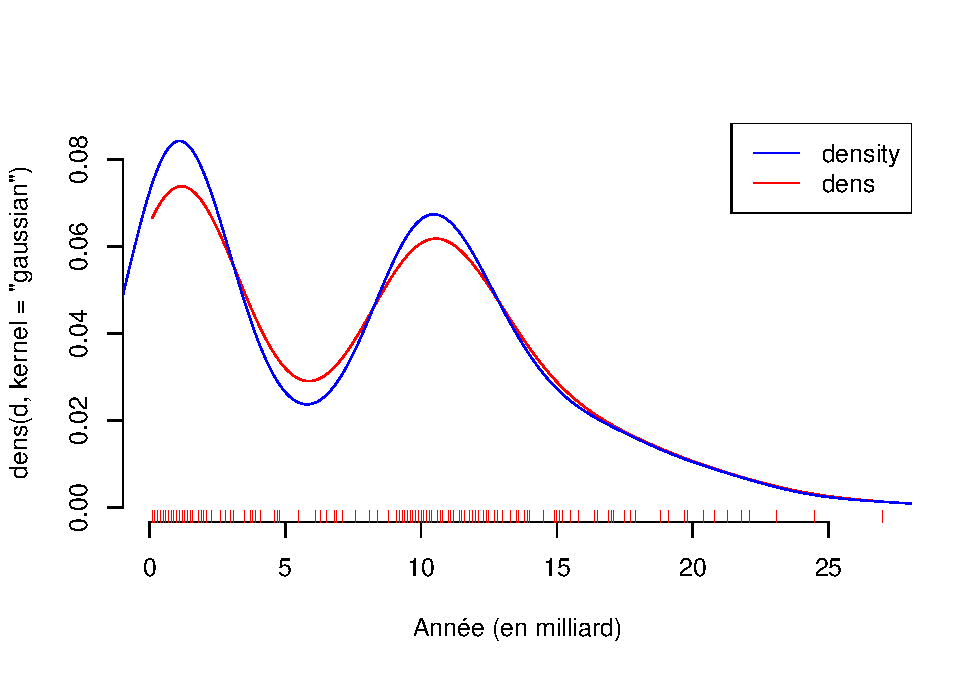
\includegraphics{Projet_M1_Chaoui_Manuel_Sadio_files/figure-latex/birds-3.pdf}

\begin{Shaded}
\begin{Highlighting}[]
\KeywordTok{cat}\NormalTok{(}\StringTok{"La moyenne de cet échantillon est de : "}\NormalTok{, }\KeywordTok{mean}\NormalTok{(d), }\StringTok{"}\CharTok{\textbackslash{}n}\StringTok{"}\NormalTok{)}
\end{Highlighting}
\end{Shaded}

\begin{verbatim}
## La moyenne de cet échantillon est de :  7.413653
\end{verbatim}

\begin{Shaded}
\begin{Highlighting}[]
\KeywordTok{cat}\NormalTok{(}\StringTok{"La variance de cet échantillon est de : "}\NormalTok{, }\KeywordTok{var}\NormalTok{(d)}\OperatorTok{*}\StringTok{ }\NormalTok{(}\KeywordTok{length}\NormalTok{(d)}\OperatorTok{-}\DecValTok{1}\NormalTok{)}\OperatorTok{/}\KeywordTok{length}\NormalTok{(d))}
\end{Highlighting}
\end{Shaded}

\begin{verbatim}
## La variance de cet échantillon est de :  38.35033
\end{verbatim}

\begin{Shaded}
\begin{Highlighting}[]
\CommentTok{# estimateur biaisé}
\CommentTok{# max(d) = 27}
\end{Highlighting}
\end{Shaded}

Sur cette échantillon on remarque une répartition bimodale de l'effectif. Effectivement, on observe un mode autour de 1 et un autre autour de 10. On peut supposer en regardant ce tableau que cet échantillon contient des familles d'oiseaux distinctes, ayant suffisamment de différences pour ne pas avoir le même temps d'évolution. C'est pour cela que la moyenne de l'échantillon se trouve au final, là où il y a peu d'individus (moins de \(5\%\)). On remarque aussi que les durée sont relativement concentrées avec une variance de \(38\), elles ne dépassent pas 27.

Maintenant, faisons une autre estimation de la densité sur un échantillon d'espèces de tortues (\texttt{chelonia}).

\begin{Shaded}
\begin{Highlighting}[]
\CommentTok{### test avec chelonia (turtules)}

\CommentTok{#### arbre}
\KeywordTok{data}\NormalTok{(chelonia)}
\NormalTok{op <-}\StringTok{ }\KeywordTok{par}\NormalTok{()}
\KeywordTok{par}\NormalTok{(}\DataTypeTok{cex =} \FloatTok{0.3}\NormalTok{)}
\KeywordTok{plot}\NormalTok{(chelonia}\OperatorTok{$}\NormalTok{phy)}
\end{Highlighting}
\end{Shaded}

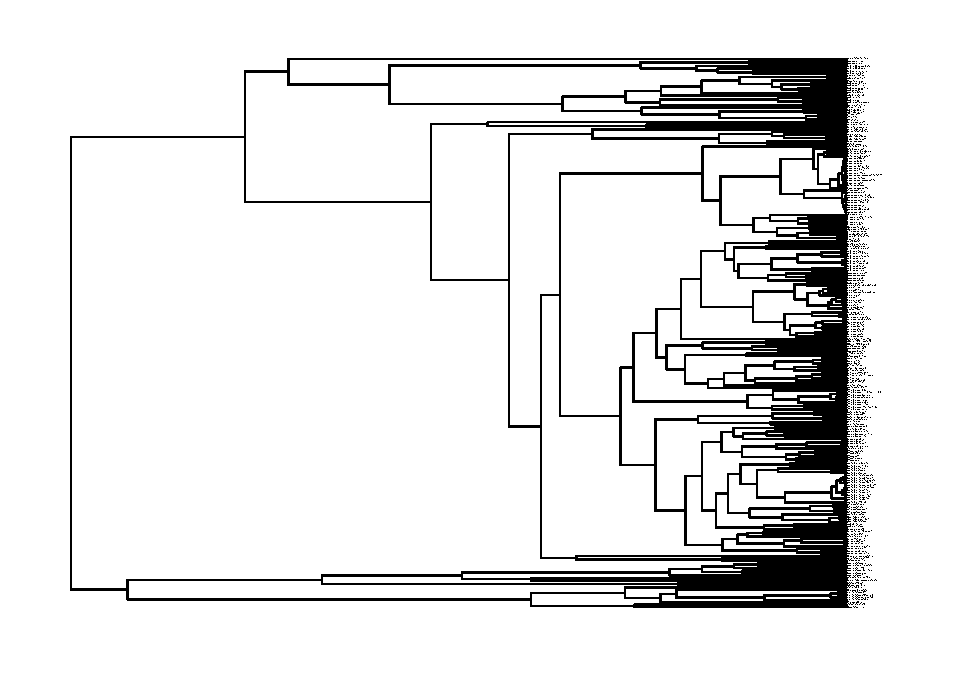
\includegraphics{Projet_M1_Chaoui_Manuel_Sadio_files/figure-latex/turtules-1.pdf}

\begin{Shaded}
\begin{Highlighting}[]
\KeywordTok{par}\NormalTok{(}\DataTypeTok{cex =}\NormalTok{ op}\OperatorTok{$}\NormalTok{cex)}

\CommentTok{#### noyau gaussien}
\NormalTok{d<-chelonia}\OperatorTok{$}\NormalTok{phy}\OperatorTok{$}\NormalTok{edge.length}
\CommentTok{#d1<-chelonia$dat}
\NormalTok{vec <-}\StringTok{ }\KeywordTok{pretty}\NormalTok{(}\DecValTok{0}\OperatorTok{:}\NormalTok{(}\KeywordTok{max}\NormalTok{(d)}\OperatorTok{+}\DecValTok{3}\NormalTok{), ((}\KeywordTok{max}\NormalTok{(d)}\OperatorTok{+}\DecValTok{3}\NormalTok{)}\OperatorTok{*}\DecValTok{2}\NormalTok{))}
\KeywordTok{hist}\NormalTok{(d, }\DataTypeTok{breaks=}\NormalTok{ vec, }\DataTypeTok{freq =}\NormalTok{ F, }\DataTypeTok{xlab =} \StringTok{"Durée"}\NormalTok{)}
\KeywordTok{lines}\NormalTok{(}\KeywordTok{density}\NormalTok{(d), }\DataTypeTok{col =} \StringTok{"red"}\NormalTok{) }\CommentTok{# bw = 0.201}
\end{Highlighting}
\end{Shaded}

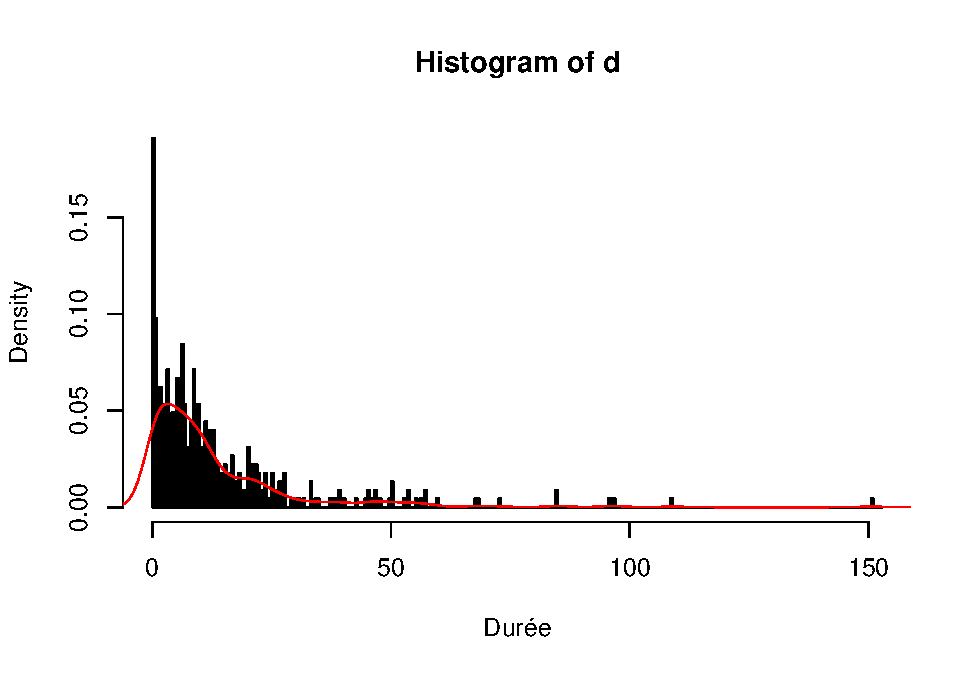
\includegraphics{Projet_M1_Chaoui_Manuel_Sadio_files/figure-latex/turtules-2.pdf}

\begin{Shaded}
\begin{Highlighting}[]
\KeywordTok{plot}\NormalTok{(}\KeywordTok{density}\NormalTok{(d, }\DataTypeTok{kernel=} \StringTok{"gaussian"}\NormalTok{), }\DataTypeTok{col =} \StringTok{"red"}\NormalTok{, }\DataTypeTok{bty =} \StringTok{"n"}\NormalTok{)}
\KeywordTok{polygon}\NormalTok{(}\KeywordTok{density}\NormalTok{(d, }\DataTypeTok{kernel=} \StringTok{"gaussian"}\NormalTok{),}\DataTypeTok{col=}\DecValTok{2}\NormalTok{,}\DataTypeTok{border =} \StringTok{"blue"}\NormalTok{)}
\KeywordTok{rug}\NormalTok{(d, }\DataTypeTok{col=} \StringTok{"red"}\NormalTok{)}
\end{Highlighting}
\end{Shaded}

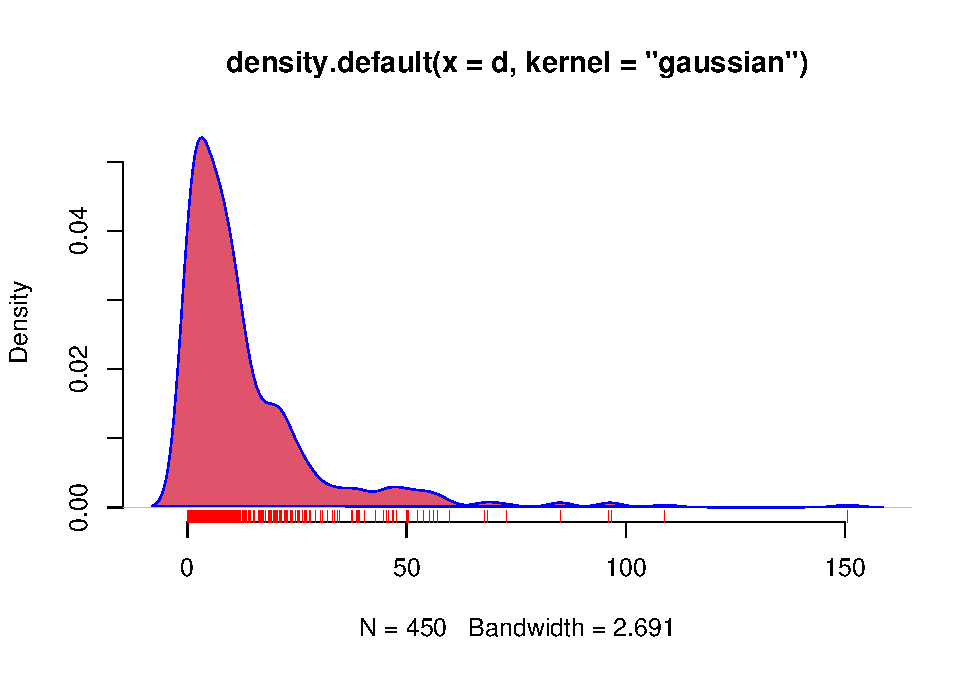
\includegraphics{Projet_M1_Chaoui_Manuel_Sadio_files/figure-latex/turtules-3.pdf}

\begin{Shaded}
\begin{Highlighting}[]
\KeywordTok{cat}\NormalTok{(}\StringTok{"La moyenne de cet échantillon est de : "}\NormalTok{, }\KeywordTok{mean}\NormalTok{(d), }\StringTok{"}\CharTok{\textbackslash{}n}\StringTok{"}\NormalTok{)}
\end{Highlighting}
\end{Shaded}

\begin{verbatim}
## La moyenne de cet échantillon est de :  12.93598
\end{verbatim}

\begin{Shaded}
\begin{Highlighting}[]
\KeywordTok{cat}\NormalTok{(}\StringTok{"La variance de cet échantillon est de : "}\NormalTok{, }\KeywordTok{var}\NormalTok{(d)}\OperatorTok{*}\StringTok{ }\NormalTok{(}\KeywordTok{length}\NormalTok{(d)}\OperatorTok{-}\DecValTok{1}\NormalTok{)}\OperatorTok{/}\KeywordTok{length}\NormalTok{(d)) }\CommentTok{# estimateur biaisé}
\end{Highlighting}
\end{Shaded}

\begin{verbatim}
## La variance de cet échantillon est de :  285.3433
\end{verbatim}

\begin{Shaded}
\begin{Highlighting}[]
\CommentTok{# max(d) = 150}
\end{Highlighting}
\end{Shaded}

Si on compare cet échantillon avec le précédent, on remarque cette fois la distribution est plus étalée (avec une variance de \(258.3\)) et unimodale. Cependant la moyenne n'est pas énormément supérieure à celle des familles d'oiseaux. Cela s'explique par le fait que beaucoup d'espèces de tortue sont apparues en moins de 25 ans et qu'on observe le pic autour de \(1\).
On en déduit qu'en moyenne on met plus de temps à obtenir une nouvelle espèce de tortue plutôt qu'une nouvelle espèce d'oiseau.

\hypertarget{conclusion}{%
\chapter{Conclusion}\label{conclusion}}

\hypertarget{references}{%
\chapter{References}\label{references}}

\label{eq:oracle} Lucie Montuelle. Inégalités d'oracle et mélanges. Statistiques {[}math.ST{]}. Université Paris-Sud, 2014.
Français.\newline
\label{eq:est-ad} Gilles Rebelles. Sur l'estimation adaptative d'une densité multivariée sous l'hypothèse de la structure d'indépendance.\newline
\label{eq:cours-est} Cours-Estimation de densité.https://cedric.cnam.fr/vertigo/Cours/ml/coursEstimationDensite.html\newline

\texttt{\textquotesingle{}\ \#\ References\ \{-\}\ \textquotesingle{}}

  \bibliography{book.bib}

\end{document}
